%************************************************
\chapter{Introduction}\label{ch:introduction}
%************************************************

Powerful modern automated theorem provers are widely used now to prove security and safety properties of computer systems.
These tools are capable of handling complex logical reasoning tasks with a degree of automation and efficiency that complements or extends manual mathematical proof development.
Their ability to automatically generate and check formal proofs has made them indispensable for ensuring the reliability and safety of both hardware and software systems, where correctness is paramount.

Satisfiability Modulo Theories (SMT) solvers \cite{cvc5,verit} are automated reasoning (AR) tools that have become especially essential in a wide range of formal reasoning tasks, including program verification and interactive theorem proving.
Their efficiency and expressive power enable them to handle complex logical proofs and verifications with speed.
At the same time, the growing reliance on SMT solvers raises a fundamental question of trust: \textit{can we be confident that the results produced by these highly complex SMT solvers are correct?}

Despite their central role, SMT solvers are large software systems with complex architectures \cite{cvc5}, often comprising hundreds of thousands of lines of code.
This complexity makes it extremely difficult to guarantee their correctness.
The annual SMT-COMP competition \cite{smtcomp2015–2018,SMT-COMP}, regularly uncovers cases where different solvers disagree on the satisfiability status of the same benchmark.
State-of-the-art SMT solvers have been found to have bugs \cite{bugsmt} due in part to error-prone optimizations, despite the best efforts of developers.
Such discrepancies highlight the practical risk of relying blindly on solver outputs in safety critical applications.

A natural response to this problem is to attempt the certification of the solver itself.
However, formally verifying such a large and complex codebase is highly impractical \cite[\S 2.2.1]{formal-method-book}.
Simplifying a solver’s design to ease certification would necessarily come at the expense of performance, which is a key factor in their adoption.
Moreover, certification tends to ``freeze'' the implementation: once a system is verified, the integration of new features, heuristics, or optimizations becomes prohibitively costly, since each change would require a new certification effort.
Consequently, directly certifying solvers in a late lifecycle of development might not scale with the pace of their development.

A first alternative is to develop a certified solver in a proof assistant environment such as the IsaSAT solver \cite{fleury:tel-02963301,fleury:hal-01904647} that is a fully verified SAT solver developed in Isabelle/HOL \cite{isabelle-hol-ref}.
This alternative offers strong guarantees about the correctness of the implementation itself, since the solver is extracted from a machine-checked formalization.
Moreover, it has been demonstrated to achieve competitive performance in SAT solving \cite{EDA-challenge}.
In this respect, IsaSAT advances the state of the art by providing a verified implementation of SAT solving.
However, the restriction to SAT limits its applicability in domains where SMT theories reasoning is required.


A second alternative line of research is \emph{proof logging} \cite{proof-logging}, where the approach is to certify the \emph{results} rather than the solver implementation.
Proof logging is a technique for automatically reviewing the reasoning steps of a proof engine by a separate tool.
This is achieved by requiring the solver to produce a proof, or certificate, of its output.
A proof trace or, more generally, certificate formally records the logical reasoning that leads to a solution, enabling independent verification by a separate proof checker.
Essentially, the task of proof checking is conceptually simpler and typically much faster than solving itself.
Moreover, a well designed trace format allows traces to be generated and checked with low performance overhead.
This decouples the trust in solver results from the correctness of the solver’s implementation, thereby providing a more practical path toward trustworthy automated reasoning.
It is then the checker of the proof trace that becomes the critical link for establishing confidence in the correctness of a verdict, and establishing soundness of a proof checker is much easier than verifying an SMT solver.
DRAT proofs \cite{drat} is a standard for verifying unsatisfiability proofs emitted by modern SAT solvers.
The independent checker rupee \cite{drat-checking} verify DRAT proofs produced by modern SAT solvers.
An attractive way of building and verifying a trace checker is to have a proof assistant interpret a trace and produce a proof that is accepted by the kernel of the proof assistant.
This method is known as \emph{proof reconstruction} \cite{z3recon}.
For example, this approach has been adopted in several proof assistants that employ \emph{hammers} for discharging goals to automatic theorem provers (ATPs), including SMT solvers.
Examples include Sledgehammer \cite{Sledgehammer} for Isabelle/HOL and CoqHammer \cite{coqhammer1,coqhammer2} for Coq.
The hammer translates the conjecture and facts supplied by the user or harvested from the context to the input language of the back-end, invokes it, and, in the case of success, attempts to reconstruct the proof in the logic of the proof assistant, based on a trace of the proof found by the back-end.

Alethe \cite{alethe,alethe2} is an established SMT proof format generated by the solvers veriT \cite{verit} and cvc5 \cite{cvc5}.
As the example \cref{lst:alethe-ex-intro} shows, the format is close to SMT-LIB and facilitating proof production.
However, it lacks a stand-alone checker, which harms its usability and hinders its adoption. 
Moreover, the coarse-grained steps can be too expensive to check and lead to verification failures.

\lstinputlisting[language=SMT]{Assets/example_uf.smt2}
\begin{center}
$\lightning$
\end{center}
\lstinputlisting[language=SMT,label={lst:alethe-ex-intro},caption={An SMT problem and its Alethe proof found by cvc5.}]{Assets/example_uf.proof}


\begin{figure}[b]
    \centering
    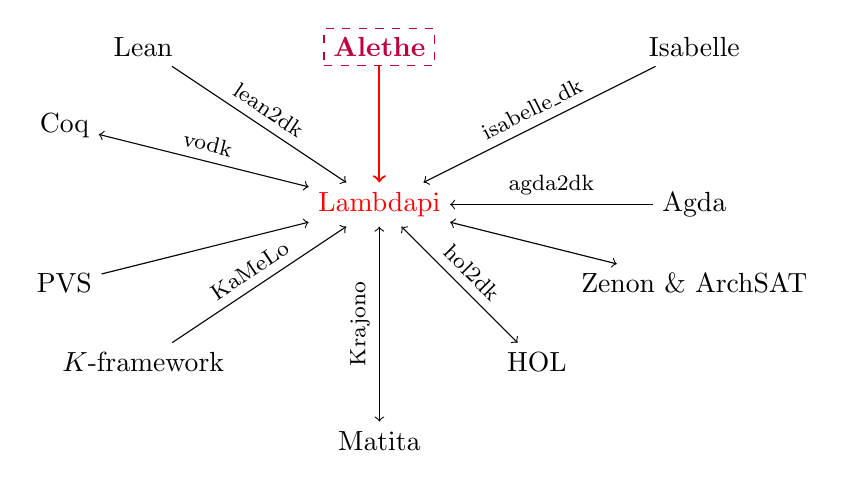
\begin{tikzpicture}
      \path (0,0) node (lp) {\textcolor{red}{Lambdapi}}
            (-4,1) node (coq) {Coq}
            (-3,2) node (lean) {Lean}
            (0,2) node [draw, dashed, purple] (smt) {\color{purple}\textbf{Alethe}}
            (4,2) node (isa) {Isabelle}
            (4,0) node (agda) {Agda}
            (-3,-2) node (k) {$\mathbb{K}$-framework}
            (0,-3) node (mat) {Matita}
            (2,-2) node (hol) {HOL}
            (-4,-1) node (pvs) {PVS}
            (4,-1) node (ze) {Zenon \& ArchSAT}
            ;
      \draw[->,red, thick] (smt) -- (lp) node[midway,sloped,above] {};
      \draw[->] (lean) -- (lp) node[midway,sloped,above] {\footnotesize{lean2dk}};
      \draw[->] (isa) -- (lp) node[midway,sloped,above] {\footnotesize{isabelle\_dk}};
      \draw[->] (agda) -- (lp) node[midway,sloped,above] {\footnotesize{agda2dk}};
      \draw[<->] (ze) -- (lp) node[midway,sloped,above] {};
      \draw[<->] (hol) -- (lp) node[midway,sloped,above] {\footnotesize{hol2dk}};
      \draw[<->] (mat) -- (lp) node[midway,sloped,above] {\footnotesize{Krajono}};
      \draw[->] (pvs) -- (lp);
      \draw[->] (k) -- (lp) node[midway,sloped,above] {\footnotesize{KaMeLo}};
      \draw[<->] (coq) -- (lp)  node[midway,sloped,above] {\footnotesize{vodk}};
    \end{tikzpicture}
    \caption{Lambdapi, an assembly language for proof systems.}
    \label{fig:interop-intro}
\end{figure}

This thesis addresses these challenges by introducing a translation framework from Alethe proofs to Lambdapi \cite{lambdapi}, a proof assistant for the $\lp$-calculus modulo rewriting ($\lpm$).
The $\lpm$-calculus combines dependent types, which enable precise encodings of object logic, with modulo theory which extends reasoning by allowing rewrite rules for defining theories and deductions.
In this way, the $\lpm$-calculus provides a meta-logic capable of expressing object logic, axioms, inference rules, and proofs of various theorem provers.
Lambdapi also supports exporting proofs to other systems (\cref{fig:interop-intro}), providing a bidirectional connection between different proof environments.
This has been one of our principal reasons for selecting Lambdapi, since it enables the conversion and sharing of Alethe proofs with other logical systems such as Rocq and Isabelle/HOL.

In this work, we identify common challenges and develop general encoding strategies.
Based on these strategies, we present a modular encoding in Lambdapi of selected Alethe inference rules.
We then empirically evaluate the effectiveness of this approach through the automated generation of proof certificates verifiable within the Lambdapi proof assistant.

\section{Thesis outline}
\label{sec:thesis-outline}

This chapter has introduced the challenges of ensuring trustworthiness in SMT solvers, highlighting the need for verifiable proofs to address the complexity and potential incorrectness of SMT solvers.
While SMT solvers are widely used in formal methods, their outputs are often taken for granted, despite the risks of errors in large, optimised codebases.
The goal of this thesis is to provide a robust framework for certifying SMT proofs by translating them into a dependently typed setting, making them both trustworthy and portable across different proof assistants.
The thesis is structured as follows:

\begin{itemize}
\item In \cref{ch:intro-lambdapi}, we introduce Lambdapi, the foundational framework for our work.
    We present the $\lambda\Pi$-calculus modulo rewriting, its typing system, and key features, including rewrite rules and inductive types.
    This chapter establishes the formal basis for encoding SMT proofs.
    It demonstrates why Lambdapi is uniquely suited for this task due to its interoperability with other proof assistants and its support for user-defined rewriting.

\item In \cref{ch:smt}, we provide background on Satisfiability Modulo Theories (SMT), covering the SMT-LIB standard, the semantics of first-order logic with theories, and the architecture of modern SMT solvers.
We discuss the role of proof production in ensuring solver correctness and motivate the need for a standardised, verifiable proof format like Alethe.

\item In \cref{ch:alethe}, we dive into the Alethe proof format, detailing its design, syntax, and logical rule system including resolution, quantifier instantiation, and theory specific rules (e.g., for linear arithmetic).
We explain how Alethe represents proofs as sequences of steps.
This chapter also highlights the challenges posed by coarse-grained proof steps and the lack of a standalone checker, which our work addresses.

\item In \cref{ch:elab}, we describe how preprocessing tools, such as Carcara \cite{carcara} and RARE \cite{rare}, refine and elaborate proofs before translation, eliminating redundant steps and preparing them for reconstruction in Lambdapi.

\item In \cref{ch:relatedworks}, we survey related work, comparing Alethe with other proof formats (e.g., Eunoia) and discussing existing approaches to integrating SMT solvers with proof assistants.
    We position our work within the broader landscape of proof certification for smt solvers.

\item In \cref{ch:encoding}, we lay the groundwork for our encoding by defining how SMT logic can be represented in Lambdapi.
    We develop a prelude that captures SMT-LIB's sorts, terms, and formulas, and show how to encode theories like Linear Integer Arithmetic (LIA) and Linear Arithmetic (LA).
    This chapter bridges the gap between SMT's many-sorted first-order logic and Lambdapi's dependent types.

\item In \Cref{ch:reconstruction}, \ref{ch:reconstruction-ul} and \ref{ch:reconstruction-la}, we present the core of our reconstruction methodology.
    The \cref{ch:reconstruction-ul} focuses on reconstructing first-order proofs, including tautologies, resolution, and quantifier handling, while \cref{ch:reconstruction-la} extends this to linear arithmetic proofs.
    We introduce reflective techniques for normalising arithmetic expressions and prove the correctness of our translations, ensuring that reconstructed proofs faithfully represent the original SMT reasoning.

\item In \cref{ch:soundness}, we formalise the correctness of our translation, proving that the encoding preserves semantic entailment.
    This chapter provides the theoretical guarantees that underpin our approach.

\item In \cref{ch:evaluation}, we shift to practical evaluation, presenting benchmarks and case studies that demonstrate the efficiency and scalability of our method.
    We show how our toolchain can validate proofs from real-world applications, including TLAPS proofs \cite{tla-proofs}, and discuss optimisations for parallel checking.

\item Finally, in Chapter~\cref{ch:conclusion}, we conclude by summarising our contributions and discussing limitations and future directions.
    We highlight the potential for extending our work to additional theories (e.g., bit-vectors) and integrating with more proof assistants, ultimately aiming to establish Alethe as a standard for proof exchange in formal methods.
\end{itemize}
